\chapter{Mendelian Randomization}
\label{ch-mendelian-rand}

Mendelian Randomization (MR)
is an application 
of the method of Instrumental Variables (IVs)
to genetics. It's 
considered an ``observational study". It's used as a
substitute  to an RCT (i.e., experimental study), when an
RCT can't be done.

IVs are discussed in Chapter \ref{ch-instrumental}.
Here is a quick review of the
essential points of that chapter.


\begin{figure}[h!]
$$
\xymatrix{
&&\rvu\ar@{-->}[dl]_\nu\ar@{-->}[dr]^\mu
\\
\rva\ar[r]_\alpha
&\rvd\ar[rr]_\delta
&&\rvy
}$$
\caption{MR assumes this bnet}
\label{fig-mend-bnet}
\end{figure}

\begin{figure}[h!]
\centering
\includegraphics[width=2in]
{mendelian-rand/mend-parallel-lines.png}
\caption{Pictorial representation of 
$ATE=y(1)-y(0)=\delta$.}
\label{fig-mend-parallel-lines}
\end{figure}

The bnet of Fig.\ref{fig-mend-bnet}
obeys the following equations:
\beq
\left\{
\begin{array}{l}
\rvy = \delta \rvd + \mu\rvu + \rvu_y
\\
\rvd = \alp\rva + \nu \rvu + \rvu_d
\end{array}
\right.
\eeq
where $\rvu_y$ and $\rvu_d$
are external, uncorrelated noises.

For any random variable
$\rvx$, define
\beq
\pder{\;\cdot}{\rvx}=
\frac{\av{\rvx, \cdot}}
{\av{\rvx, \rvx}}
\;.
\eeq

If one solves for 
$\delta$, one gets

\beq
ATE = \delta =
\frac{\pder{\rvy}{\rva}}
{\pder{\rvd}{\rva}}
\eeq
This formula for 
$\delta$ 
can be estimated 
using Linear Regression.
See Fig.\ref{fig-mend-parallel-lines}
for a pictorial
representation of $\delta$.

\hrule\noindent What these random variables stand for in MR:

$\rva:$ genotype (inherited genetic variant trait).
This is the IV.

$\rvu:$ hidden variable, ``confounders" (good
controls) 


$\rvd\in\bool$: exposure

$\rvy\in\bool$: outcome 

\hrule
\noindent  Example

$\rva:$ has genotype
that is strongly associated with heavy smokers?

$\rvu:$ city dweller?


$\rvd$: smoker?

$\rvy$: died of lung cancer?



\hrule\noindent{\bf Assumptions of MR (should be tested)}

\begin{itemize}
\item $\rva\rarrow \rvd$, but
no $\rva\rarrow \rvy$
\item
no confounder $\rvc$ such that $\rvc\rarrow \rva, \rvy$ 
\item 
no feedback
(a.k.a. reverse causation) arrows $\rvy\rarrow \rva$.
\end{itemize}

Using genotype for $\rva$ makes
these assumptions more likely.
